\documentclass[10pt]{article}
\usepackage{../../local}


\newcommand{\classcode}{Physics 105}
\newcommand{\classname}{Analytic Mechanics}
\renewcommand{\maketitle}{%
\hrule height4pt
\large{Eric Du \hfill \classcode}
\newline
\large{HW 06} \Large{\hfill \classname \hfill} \large{\today}
\hrule height4pt \vskip .7em
\normalsize
}
\linespread{1.1}
\begin{document}
	\maketitle
	\section*{Collaborators}

	I worked with \textbf{Andrew Binder, Adarsh Iyer} and \textbf{Aren Martinian} to complete this homework.

	\section*{Problem 1}
	A bucket of water is set spinning about its symmetry axis with angular speed $\Omega$. Determine the shape
	of the water in the bucket.

	\begin{solution}
		Consider a small portion of mass $m$. The centrifugal force acting on it $F_{cf} = m\Omega^2 \rho \hat{
		\rho}$, and the gravitational force is $F_g = -mg \hat{z}$. Therefore, using $\nabla U = -F$, we know
		that:
		\[
		U = mgz -\frac{1}{2} m \Omega^2 \rho^2
		\] 
		We now use the fact that the surface of the water is an equipotential, so we require $U$ to be constant.
		Deriving a relation for $z$ in terms of $\rho$, we get:
		\begin{align*}
			mgz &= U + \frac{m \Omega^2 r^2}{2}\\
			z(r) &= \frac{2U + m \Omega^2 \rho^2}{2mg}
		\end{align*}
		which means that $z \propto \rho ^2$ implying that the shape of the water surface is that of a parabola. 
	\end{solution}

	\pagebreak
	\section*{Problem 2}
	A car is driving with acceleration $a$ and instantaneous velocity $v$. The tires of radius $r$ are not 
	slipping. What point on the tire has the greatest acceleration relative to the ground? What is this 
	acceleration?

	\begin{solution}
		Consider the following diagram: 
		
		\begin{center}
			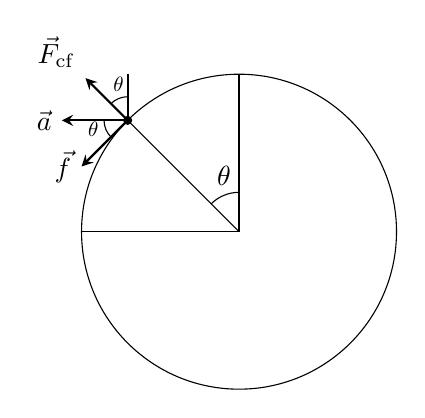
\begin{tikzpicture}
            \draw (0,0) circle (2cm);
            \draw (0,0) -- (0,2);
            \draw (0,0) -- (-2,0);
            \draw (0,0) -- (-1.414,1.414);
            \draw (0,0.5) arc (90:135:0.5cm) node[midway, above] {$\theta$};
            \filldraw[black] (-1.414,1.414) circle (0.05cm);
            \draw[thick, -stealth] (-1.414,1.414) -- (-2,0.828) node[anchor=east] {$\vec{f}$};
            \draw[thick, -stealth] (-1.414,1.414) -- (-1.95,1.95) node[anchor=south east] {$\vec{F}_{\mathrm{cf}}$};
            \draw[thick] (-1.414,1.414) -- (-1.414,2);
            \draw (-1.414,1.714) arc (90:135:0.3cm) node[midway,above,scale=0.75] {$\theta$};
            \draw[thick, -stealth] (-1.414,1.414) -- (-2.25,1.414) node[anchor=east] {$\vec{a}$};
            \draw (-1.714,1.414) arc (180:225:0.3cm) node[midway,left,scale=0.75] {$\theta$};
        \end{tikzpicture}
		\end{center}

		Here, we have a friction term because the wheel is rolling without slipping. In order to maximize 
		the acceleration relative to the ground, we require that the acceleration vectors add constructively, 
		and the location at which this occurs is shown in the diagram above. Now, consider the acceleration in 
		the $y$ direction:
		\[
			a_y = F_{cf} \cos \theta - f sin \theta
		\] 
		$a_y = 0$ since the wheel isn't accelerating either up or down, therefore we have the equation: 
		\[
			F_{cf} \cos \theta = f \sin \theta
		\] 
		Solving for $\theta$, we get:
		\begin{align*}
			tan \theta &= \frac{F_{cf}}{f} = \frac{m\Omega^2}{mrA} = \frac{\Omega^2}{A} = \frac{v^2}{rA}\\
			\therefore \theta &= \tan^{-1}\left( \frac{v^2}{rA} \right) 
		\end{align*}

		Here, I use $A$ to reference the linear acceleration of the car. This acceleration exists only in the $
		x$ direction now:
		\begin{align*}
			a_x &= F_{cf} \sin \theta + f \cos \theta + a\\
				&= m\Omega^2 r \sin\left( \tan^{-1}\left( \frac{v^2}{rA} \right)  \right)  + f \cos \left( 
				\tan^{-1}\left( \frac{v^2}{rA} \right) \right) +a
		\end{align*}
		which is also the total magnitude of the acceleration.
	\end{solution}


	\pagebreak
	\section*{Problem 3}
	How much greater is the acceleration due to Earth's gravity $g$ at the equator than at the pole (assume a 
	spherical Earth)? If the actual measured difference is $\Delta g = 52 \ \mathrm{mm/s^2}$, explain this 
	difference. How might you calculate this difference between the measured result and your calculation?

	\begin{solution}
		The net force on an object on Earth is $F = F_g + F_{cf} + F_{cor}$. Since we are measuring the 
		acceleration relative to ourselves, $F_{cor} = 0$. Furthermore, an observer at the north pole experiences
		no Coriolis force, so therefore the gravity it experiences is simply $F_g$. Therefore, we have the
		equation:
		\begin{align*}
			m\ddot r &= mg - m\Omega^2 \rho \\
			\therefore \ddot r &= 9.8 \mathrm{m/s^2} - \Omega^2 r_e
		\end{align*}
		Crunching the numbers, we get that $\Omega^2 r_e = 0.034 \ \mathrm{m/s^2}$, or $34 \ \mathrm{mm/s^2}$.
		To explain the difference between the measured result and this calculation, we have to remember that 
		the Earth is not exactly a sphere, and its radius is larger at the equator than at the pole, so we'd 
		expect a larger discrepancy. To calculate this difference, it suffices to look at the difference between
		the magnitude of the centrifugal force on a spherical Earth as opposed to an ellipsoidal one, since
		the mass in both scenarios is the same. 
	\end{solution}

	\pagebreak
	\section*{Problem 4}
	Supposedly, during World War I, there was an event during which a British warship near the Falkland Islands
	repeatedly missed its target due to not accounting for the Coriolis force. If it fires a projectile due 
	South at latitude $50^\circ$S at $33^\circ$ elevation with a speed of 800  m/s, by how much do the shells
	miss their target and in what direction? Ignore air resistance. 

	\begin{solution}
		We set up our coordinate axes as follows:

		\begin{center}
			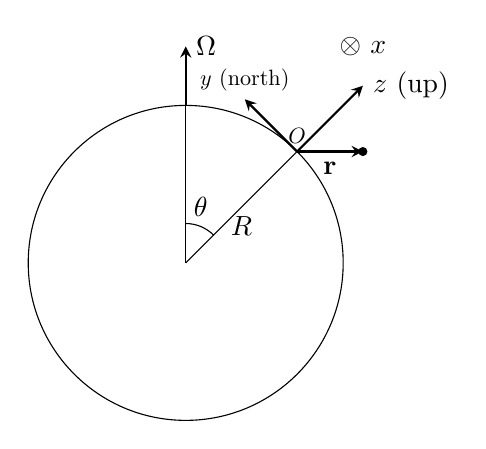
\begin{tikzpicture}
            \draw (0,0) circle (2cm);
            \draw (0,0) -- (0,2);
            \draw (0,0) -- (1.414,1.414) node[midway,below] {$R$};
            \draw (0,0.5) arc (90:45:0.5cm) node[midway, above] {$\theta$};
            \draw[thick, -stealth] (0,2) -- (0,2.75) node[anchor=west] {$\boldsymbol{\Omega}$};
            \draw[thick, -stealth] (1.414,1.414) -- (2.25,1.414) node[midway, below] {$\mathbf{r}$};
            \filldraw[black] (2.25,1.414) circle (0.05cm);
            \draw[thick, -stealth] (1.414,1.414) node[anchor=south,scale=0.8] {$O$} -- (2.25,2.25) node[anchor=west] {$z$ (up)};
            \draw[thick, -stealth] (1.414,1.414) -- (0.75,2.078) node[anchor=south,scale=0.8] {$y$ (north)};
            \node at (2.25,2.75) (x) {$\otimes$ $x$};
        \end{tikzpicture}
	\end{center}	
		The equations of motion for a particle which subject to the Coriolis force is:
		\begin{align*}
			\ddot x &= 2\Omega(\dot y \cos \theta - \dot z \sin \theta) \\
			\ddot y &= -2\Omega \dot x \cos \theta \\
			\ddot z &= -g + 2\Omega x \sin \theta
		\end{align*}
		These are the general equations of motion, without any approximations. From the problem statement, we 
		know that:
		\begin{align*}
			\dot y &= -800 \cos (33^\circ) & \dot z &= 800\sin(33^\circ) - gt \\
			\ddot y &= 0 & \ddot z &= -g \\
		\end{align*}
		So substituting this into our equation for $\ddot x$, we get: 
		\[
		\ddot x = 2\Omega(-800 \cos(33^\circ) \cos (140^\circ) - (800 \sin(33^\circ) - gt)\sin(140^\circ)
		\] 
		Integrating twice, we get the equation (and also evaluating the known terms):
		\[
		x(t) = \frac{467.82\Omega}{2}t^2 + \frac{12.6 \Omega}{6}t^3
		\] 
		All that remains now is to find the time of flight $t$. To do this, we use our equations of projectile
		motion. Since the Coriolis force acts perpendicularly to the velocity of the particle at all times, then
		its presence does not affect the projectile's time of flight. Therefore, using standard equations for 
		projectile motion, we know that: 
		\[
		 T = \frac{2v_0\sin \theta}{g} = 88.92 \text{ seconds}
		\] 
		Plugging this time back into $x(t)$, gives:
		\[
		x(t =88.92) = 241.79 \text{ m}
		\] 
		which is the distance travelled east due to the Coriolis force. 
	\end{solution}

	\pagebreak
	\section*{Problem 5}
	Show that the equation motion of a particle of mass $m$ with spatial coordinate $\mathbf r$ and velocity 
	$\mathbf v$ in a noninertial reference frame can be written in the form of the Euler-Lagrange equation with a
	potential given by 
	\[
		V = -m\mathbf{\Omega} \times \mathbf{r \cdot v} + m\mathbf{A \cdot r} - \frac{m}{2}(\mathbf{\Omega \times
		r})^2
	\] 
	where $\mathbf A$ is the frame's linear acceleration and $\mathbf \Omega$ is its angular velocity vector. 

	\begin{solution}
		We write out our Lagrangian: 
		\[
			\mathcal L = T - U = \frac{1}{2}m \mathbf r^2 + m(\mathbf{\Omega \times r}) \cdot \mathbf r - m
			\mathbf{A \cdot r} + \frac{m}{2}(\mathbf{\Omega \times r})^2
		\] 
		Taking the derivative with respect to $\mathbf r$, we get: 
		\[
		\pdv{\mathcal L}{\mathbf r} = m(\mathbf{\dot r \times \Omega}) - m\mathbf A + m\mathbf{\Omega}^2 \mathbf
		r
			- m(\mathbf{\Omega \cdot r}) \mathbf{\Omega}
		\] 
		Now with respect to $\dot{\mathbf r}$:
		\[
			\pdv{\mathcal L}{\dot{\mathbf r}} = m\dot{\mathbf r} + m(\mathbf{\Omega \times r}) 
		\] 
		so: 
		\[
			\dv{t}\left( \pdv{\mathcal L}{\dot{\mathbf r}} \right) = m\ddot{\mathbf r} + m(\mathbf{\Omega \times
			r})
		\] 
		Putting these together, we get: 
		\begin{align*}
			m\ddot{\mathbf r} + m(\mathbf{\Omega \times r}) &= m(\mathbf{r \times \Omega}) - m\mathbf A + m
			\underbrace{\mathbf{\Omega}^2 \mathbf r - m(\mathbf{\Omega \cdot r})\mathbf \Omega}_{= m(\mathbf{
			\Omega \times r}) \times \mathbf \Omega}\\
			\therefore m\ddot{\mathbf r} &= 2m(\mathbf(r \times \Omega) - m\mathbf A +
			m(\mathbf{\Omega \times r}) \times \mathbf{\Omega}
		\end{align*}
		as desired. 
	\end{solution}


\end{document}
